\section{Introduction}
\label{sec-intro}

%Nowadays, many applications involve with relations between more than one type of entities, and their data are always recorded as heterogeneous graphs, such as the heterogeneous information graph of literature entities, where  scholarly articles (papers) are connected with their authors, venues and affiliations, as well as other articles as references. Assessing the importance of nodes in (heterogeneous) graphs is one of the most essential tasks, which may find useful in many other scenarios.

Query independent ranking of scholarly articles has drawn significant attentions from both academia~\cite{Garfield471,ChenXMR07,Zhou07-CoRank,ShenAAAI16,Liang16AAAI,Jiang12-MRank,Waltman2014,TanLMGSW16} and industry~\cite{sem-scholar,g-scholar,Sinha15:MAG}. Generally speaking, a ranking is {\em a function that assigns each entity a numerical score}. Query independent ranking aims to give a static ranking based on the scholarly article data only, and is independent of how well articles match a specific query. Such a ranking plays a key role in literature recommendation systems, especially in the {\em cold start} scenario.

\eat{
In this work, we focus on ranking the importance of scholarly articles in a query independent way, which has drawn significant attentions from both academia and industry. In the academic community, the most popular approaches to scholarly article ranking have witnessed a shift from citation count analysis~\cite{Garfield471,Hirsch15112005} to graph analysis~\cite{ChenXMR07,Zhou07-CoRank,Jiang12-MRank,Waltman2014}. These graph-based methods leverage the global structure information of the bibliographic network, within which the importance is propagated and, finally, mutually reinforced between one or multiple types of entities.

In the industry, efforts have also been made to scholarly article ranking, among which Google Scholar~\cite{g-scholar}
%, Microsoft Academic Search~\cite{ms-academic}
and Semantic Scholar~\cite{sem-scholar} are the most prominent. More specifically, Google Scholar aims to rank articles in the way researchers do, weighing the full text, where it was published, who it was written by, as well as how often and how recently it has been cited.
%Microsoft Academic Search considers how often and where a publication is cited to determine the ranking.
Semantic Scholar proposes to use the citation velocity feature, which is a weighted average of the publication's citations for the last 3 years.
}

% https://scholar.google.com/intl/zh-CN/scholar/about.html
% http://academic.research.microsoft.com/About/Help.htm
% https://www.semanticscholar.org/faq#citation-velocity




Scholarly articles are involved with multiple entities such as authors, venues, dates and references. Hence, scholarly article ranking is essentially a problem of assessing the importance of nodes in a heterogeneous network.
However, effective and efficient ranking of nodes in such a large complex network is a challenging task since entities
are heterogeneous, evolving and dynamic~\cite{AggarwalS14-survey,fcs-biggraph}.



First, even if we are only to rank one type of entities (\eg scholarly articles), the other types of entities (\eg venues and authors) are closely involved, and, moreover, different types of entities may have different impacts on the ranking of scholarly articles.
%
%Second, entities are evolving, and the importance of an article varies with time~\cite{Li08TSRanking}. Newly published articles are very likely to have increasing impacts in the next few years, and those published many years ago tend to have decreasing impacts, as researchers potentially have more interests in recent reported  results. As indicated by the statistics of the Microsoft Academic Graph (\magdata)~\cite{Sinha15:MAG} in Fig.~\ref{fig-citation}, the citations of articles indeed increase in the first two years after their publication, and then decrease accordingly.
%
Second, the importance of an article varies with time~\cite{WangSB13}. Newly published articles are very likely to have increasing impacts in the next few years, and those published many years ago tend to have decreasing impacts, as researchers potentially have more interests in recently reported results. Indeed, as shown by the statistics of three scholarly datasets (\aan, \aminer and \magdata) in Fig.~\ref{fig-citation}, the citation numbers of articles in general reach the peak in the first 1 or 2 years after their publication, and then decrease accordingly. % Note that we do not plot the proportion of citations at $x=0$ on \aminer, which is an impractical value of 23.6\%. The above citation pattern is described as a complex log-normal probability in~\cite{WangSB13}.
%
Finally, academic data is dynamic and continuously growing. Indeed, the number of articles in \magdata has exceeded 126 million, and keeps increasing at around 5.7 million per year~\cite{Sinha15:MAG}.



%Managing scholarly data with such volume in  highly dynamic scenarios is a non-trivial task. However, existing methods rarely consider the efficiency issue. Moreover, incremental algorithms are necessary to manage scholarly data in highly dynamic scenarios, which are still in the early stage in the literature.
Query independent ranking of scholarly articles is challenging~\cite{wsdmcup}, although there exists quite a bit of work on scholarly article ranking, \eg~\cite{Garfield471,ChenXMR07,Zhou07-CoRank,ShenAAAI16,Liang16AAAI,Jiang12-MRank,Waltman2014}.
Further, to our knowledge, little concern has been paid to dynamic scholarly article ranking except \cite{GhoshKHLL11} with a strong and impractical assumption that there are no citations between papers published in the same years.


%Indeed, {\em how to accurately rank nodes in dynamic heterogeneous graphs remains a challenging task}.


%Furthermore, there are several study on incremental PageRank that can be employed for dynamic scholarly article ranking~\cite{DesikanPSK05,AbiteboulPC03,WuR09} Moreover, there exists little work on handing dynamic academic data except \cite{GhoshKHLL11}, although there are several study on incremental PageRank that can be employed for dynamic scholarly article ranking~\cite{DesikanPSK05,AbiteboulPC03,WuR09}



\eat{
Another concern of scholarly article ranking is to model the importance of articles that meets human expectation. Essentially, people are more interest in scholarly articles that are influential in the present and the near future, as also indicated by the ranking policies of Google Scholar~\cite{g-scholar} and Semantic Scholar~\cite{sem-scholar}. Currently, most existing graph-based methods exploit PageRank and its variants as the ranking components~\cite{Waltman2014,sayyadi09,Zhou07-CoRank}, which means importance of articles is indeed prestige voted by other articles through citations. However, as pointed out in~\cite{Li08TSRanking}, PageRank based methods favour older articles that have accumulated a large number of citations. On the other hand, recently published articles are often underestimated, even though they potentially have an increasing impact. Moreover, the prestige of articles never decreases while impacts of articles do decrease. As a result, merely modeling importance as prestige fails to give a reasonable ranking.
}




%{\bf motivate the need for dealing with dynamic scenario}.



%Currently, structure based methods, such as PageRank~\cite{Brin98:PageRank} and its variant Weighted PageRank~\cite{Xing04:WPR}, are among the most effective ones for ranking scholarly articles. However, as pointed out in~\cite{Li08TSRanking}, these previous methods favour older articles that have accumulated a large number of links (\eg citations). However, recently published articles are often underestimated, and they potentially have an increasing impact. These motivate us to develop a new approach to ranking the importance of scholarly articles.


\begin{figure}
\vspace{1ex}
\includegraphics[scale=0.45]{fig/citation.eps}
\vspace{-2ex}
\caption{\small Citation statistics of scholarly articles}
\label{fig-citation}
\vspace{-5ex}
\end{figure}


\eat{
%%%%%%%%%%%%%%%%%%%%%%%%%%%%%%%%%%%%%%%%%%%%%%%%%%
\begin{table}[t!]
%\vspace{-2ex}
\label{tab-citation}
\begin{center}
\begin{small}
\vspace{1ex}
\begin{tabular}{|c|c|c|c|c|c|c|c|c|c|c|}
\hline
$Y_p$  & 0 & 1 & 2 & 3 & 4 & 5 & 6 & 7 & 8 & 9  \\
\hline \hline
\aan  & 4.0 & {\bf 17.2} & 15.7 & 12.5 & 10.3 & 8.1 & 6.9 & 5.4 & 4.3 & 3.0     \\  \hline
\aminer  & {\bf 23.6} & 7.9 & {\bf 9.6} & 8.9 & 7.9 & 6.8 & 5.7 & 4.8 & 4.0 & 3.3      \\ \hline
\magdata & 2.5 & 7.4 & {\bf 9.3} & 8.9 & 8.0 & 7.2 & 6.4 & 5.7 & 5.0 & 4.4   \\ \hline
\end{tabular}
\vspace{-0ex}
\end{small}
\end{center}
\caption{\small proportion of citations after $Y_p$ years}
\vspace{-3ex}
\end{table}
%%%%%%%%%%%%%%%%%%%
}

\stitle{Contributions \& Roadmap}.
To this end, we propose an effective and efficient approach for query independent scholarly article ranking in a dynamic environment.

\sstab(1) We first  propose a \underline{S}cholarly \underline{A}rticle \underline{Rank}ing model, referred to as \ensemblerank, by assembling the importance of three classes of entities (articles, venues and authors) for scholarly article ranking (Section \ref{sec-model}).
%
The importance is a combination of {\em prestige} and {\em popularity} to capture the evolving nature of entities.
%
To compute the prestige of articles and venues, we propose a novel {\em Time-Weighted PageRank} with a time decaying factor (based on citation statistics), and the prestige of authors is the average prestige of all their published articles.
%
The popularity of an article is the sum of all its citations' freshness (how close to the current year), while the one of venues and authors is the average popularity of their associated articles.
%
%Observe that (a), intuitively, prestige favors articles with many citations soon after their publication, and popularity favors those with recent citations, and (b) both prestige and popularity capture the evolving nature of entities.


\sstab(2)  We then develop  a batch algorithm for scholarly article ranking (Section \ref{sec-alg}), in which we propose a block-wise method for Time-Weighted PageRank in terms of an analysis of the citation characteristics of scholarly articles.
%
We further develop an incremental algorithm for dynamic scholarly article ranking (Section~\ref{sec-incAlg}), which partitions graphs into  {\em affected and unaffected areas}, and employs different updating strategies for nodes in different areas.

%The key of our approach \ensemblerank is a good solution for Time-Weighted PageRank. As a starting point, we show a block-wise PageRank computation method is a good choice on scholarly data obeying the {\em temporal order}, \ie articles only cite existing ones .

%



\eat{
\sstab(2) We then propose an efficient batch algorithm, which exploits the {\em temporal order} of scholarly data,
\ie articles only cite previously published ones, to speed-up the computation (Section \ref{sec-alg}).
The key of our ensemble approach \ensemblerank is a good solution for Time-Weighted PageRank, whose time complexity is significantly reduced with the usage of the temporal order.
%For the prestige of articles, its time complexity is reduced to $O(|V|+|E|)$, and for the prestige of venues,  its time complexity is reduced to $O(|V|+|E|+t\cdot |E_w|)$, instead of $O(t\cdot(|V|+|E|))$. Here (a) $|V|$ and $|E|$ are the numbers of nodes and edges, (b) $|E_w|$ is the number of edges within strongly connected components and is much less than $|E|$ on scholarly data in practice, and (c) $t$ is the number of iterations.

\sstab(3) We also propose an incremental algorithm that further speeds up scholarly article ranking in a dynamic environment (Section~\ref{sec-incAlg}). The incremental algorithm is based on the division of original graphs into {\em affected and unaffected areas}, and different updating strategies are designed for nodes in affected and unaffected areas.
}

\sstab(3) Using three real-life scholarly datasets (\aan, \aminer and \magdata), we finally conduct an extensive experimental study (Section~\ref{sec-exp}).
(a) We find that our \ensemblerank model improves the pairwise accuracy \cite{Richardson06:BPR} over (\pagerank \cite{Brin98:PageRank}, \futurerank \cite{sayyadi09}, \hhgrank \cite{Liang16AAAI}) by
(14.55\%, 5.2\%, 4.65\%) on \aan,
(12.9\%, 4.5\%, 3.4\%) on \aminer and
(8.95\%, 3.3\%, 1.75\%) on \magdata, on average, respectively.
%
(b) Our batch algorithm \batensemble and incremental algorithm \incensemble are also efficient. Indeed, \incensemble is on average (2.0, 4.1, 229) times faster than (\batensemble, \futurerank, \hhgrank)  on the large dataset \magdata.

\eat{
(b) Our batch algorithm \batensemble is on average (1.3, 2.5, 348) times faster than (\powensemble, \futurerank, \hhgrank)  on the large dataset \magdata.
%
(c) Our incremental algorithm \incensemble is consistently faster than its batch counterpart \batensemble, \eg on average 22\% faster on \magdata.
}

%discusses how to deal with missing data using external sources


%All detailed proofs of this paper are available at \cite{SARank-full}.


\eat{
\stitle{Organization}. The rest of our paper is organized as follows. The latter part of Section~\ref{sec-intro} summarizes related work. Section~\ref{sec-model} introduces the ranking model. Section~\ref{sec-alg} .... Section~\ref{sec-incAlg} .... Experimental results are reported in Section~\ref{sec-exp}, followed by conclusions in Section~\ref{sec-conc}.
}



